\chapter{An algorithm for testing pattern-avoidance of a special pattern}
\label{chap:walking}
In the previous chapter, we have seen an algorithm for a general forbidden pattern which, using some heuristics, runs pretty fast. In this chapter, we introduce a special kind of a pattern, satisfying additional conditions, for which we can produce much faster algorithm.

\section{Walking pattern}
We call the specific pattern a walking pattern. The additional condition we want the pattern to satisfy is that there is a walk from one corner to the opposite one and all the one-entries of the pattern are contained on the walk.
\paragraph{Definition}
A \textbf{walk} in a matrix is a sequence of some of its entries beginning in the top left corner and ending in the bottom right one. If an entry at the position $[i,j]$ is in the sequence, the next one is either $[i+1,j]$ or $[i,j+1]$. Therefore, the length of an arbitrary walk is equal to $w+h-1$.
\begin{figure}[h!]
\centering
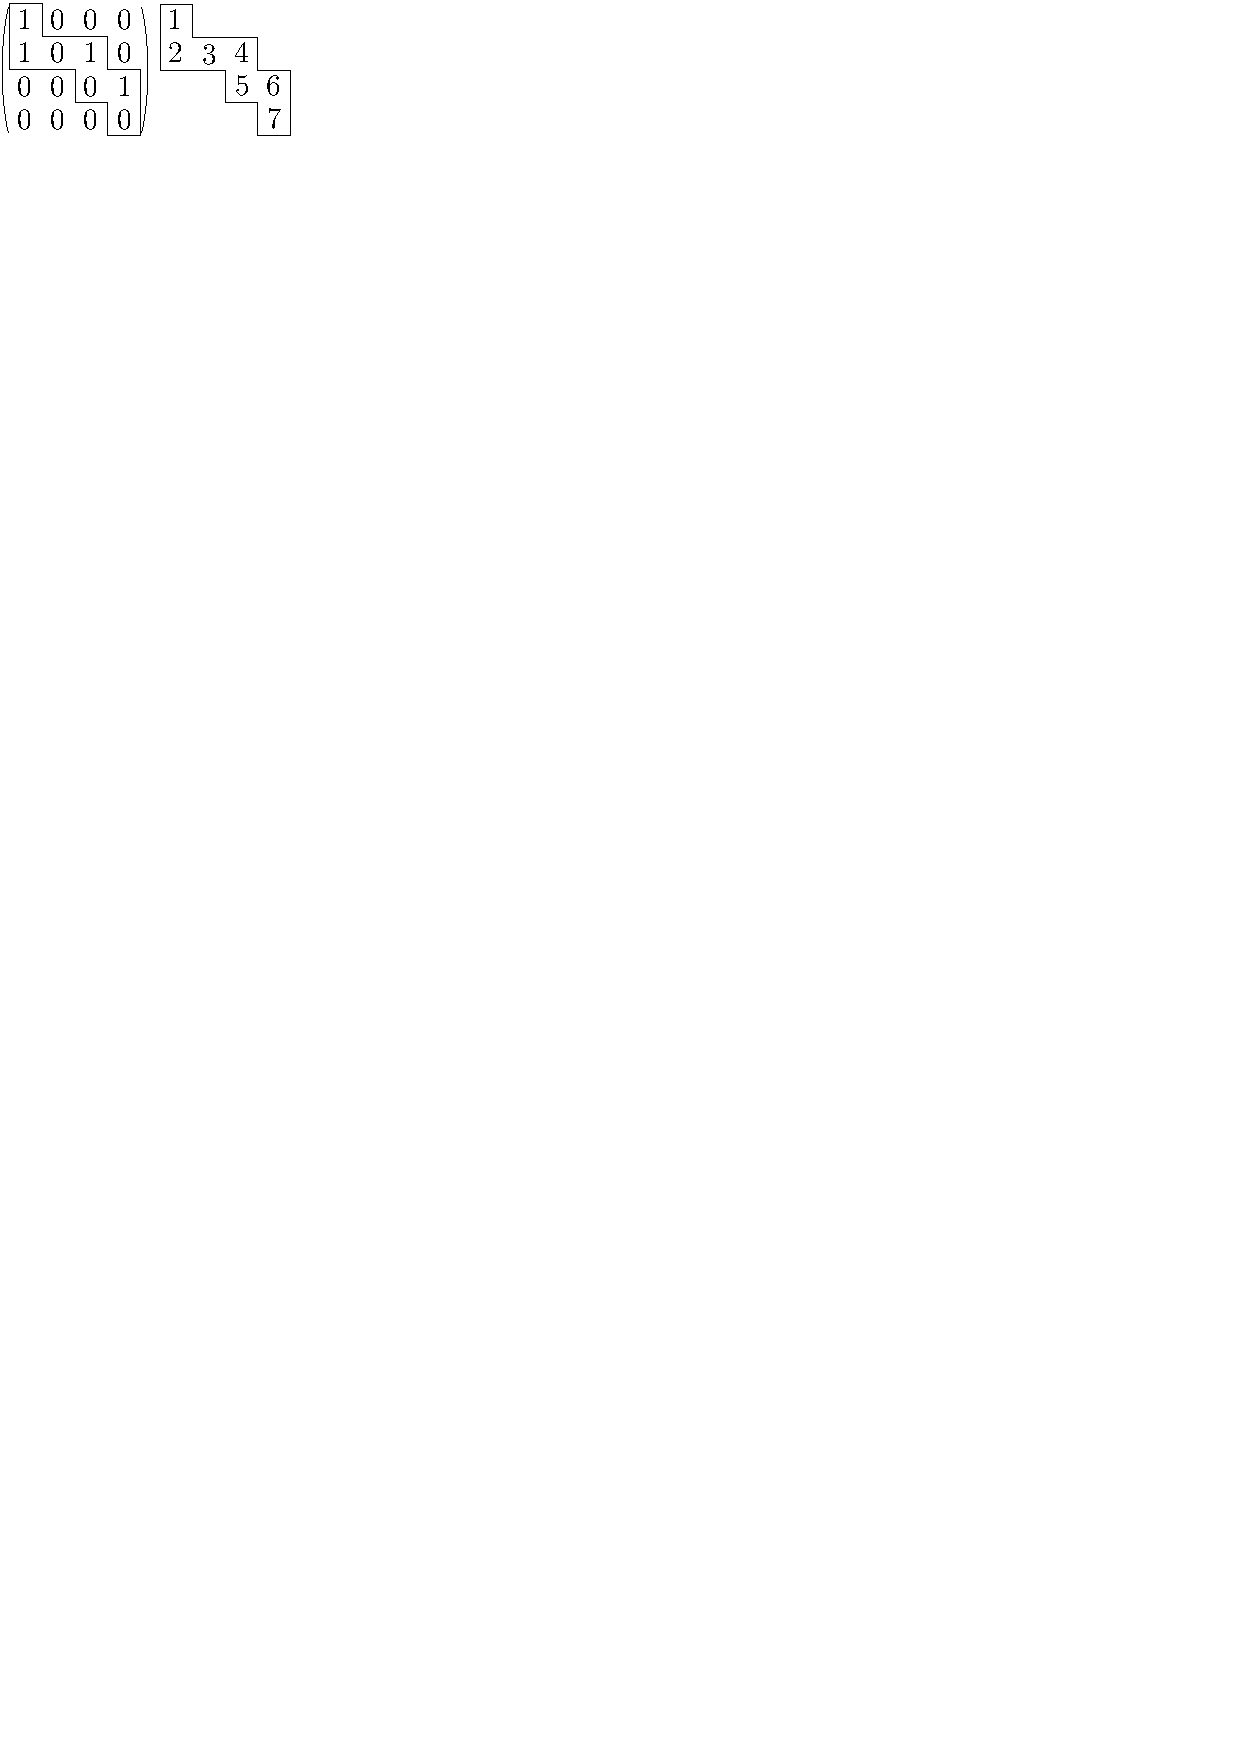
\includegraphics[width=100mm]{../img/walk.pdf}
\caption{An example of a walk and the order of its entries.}
\label{walk}
\end{figure}
%\centerline{\mbox{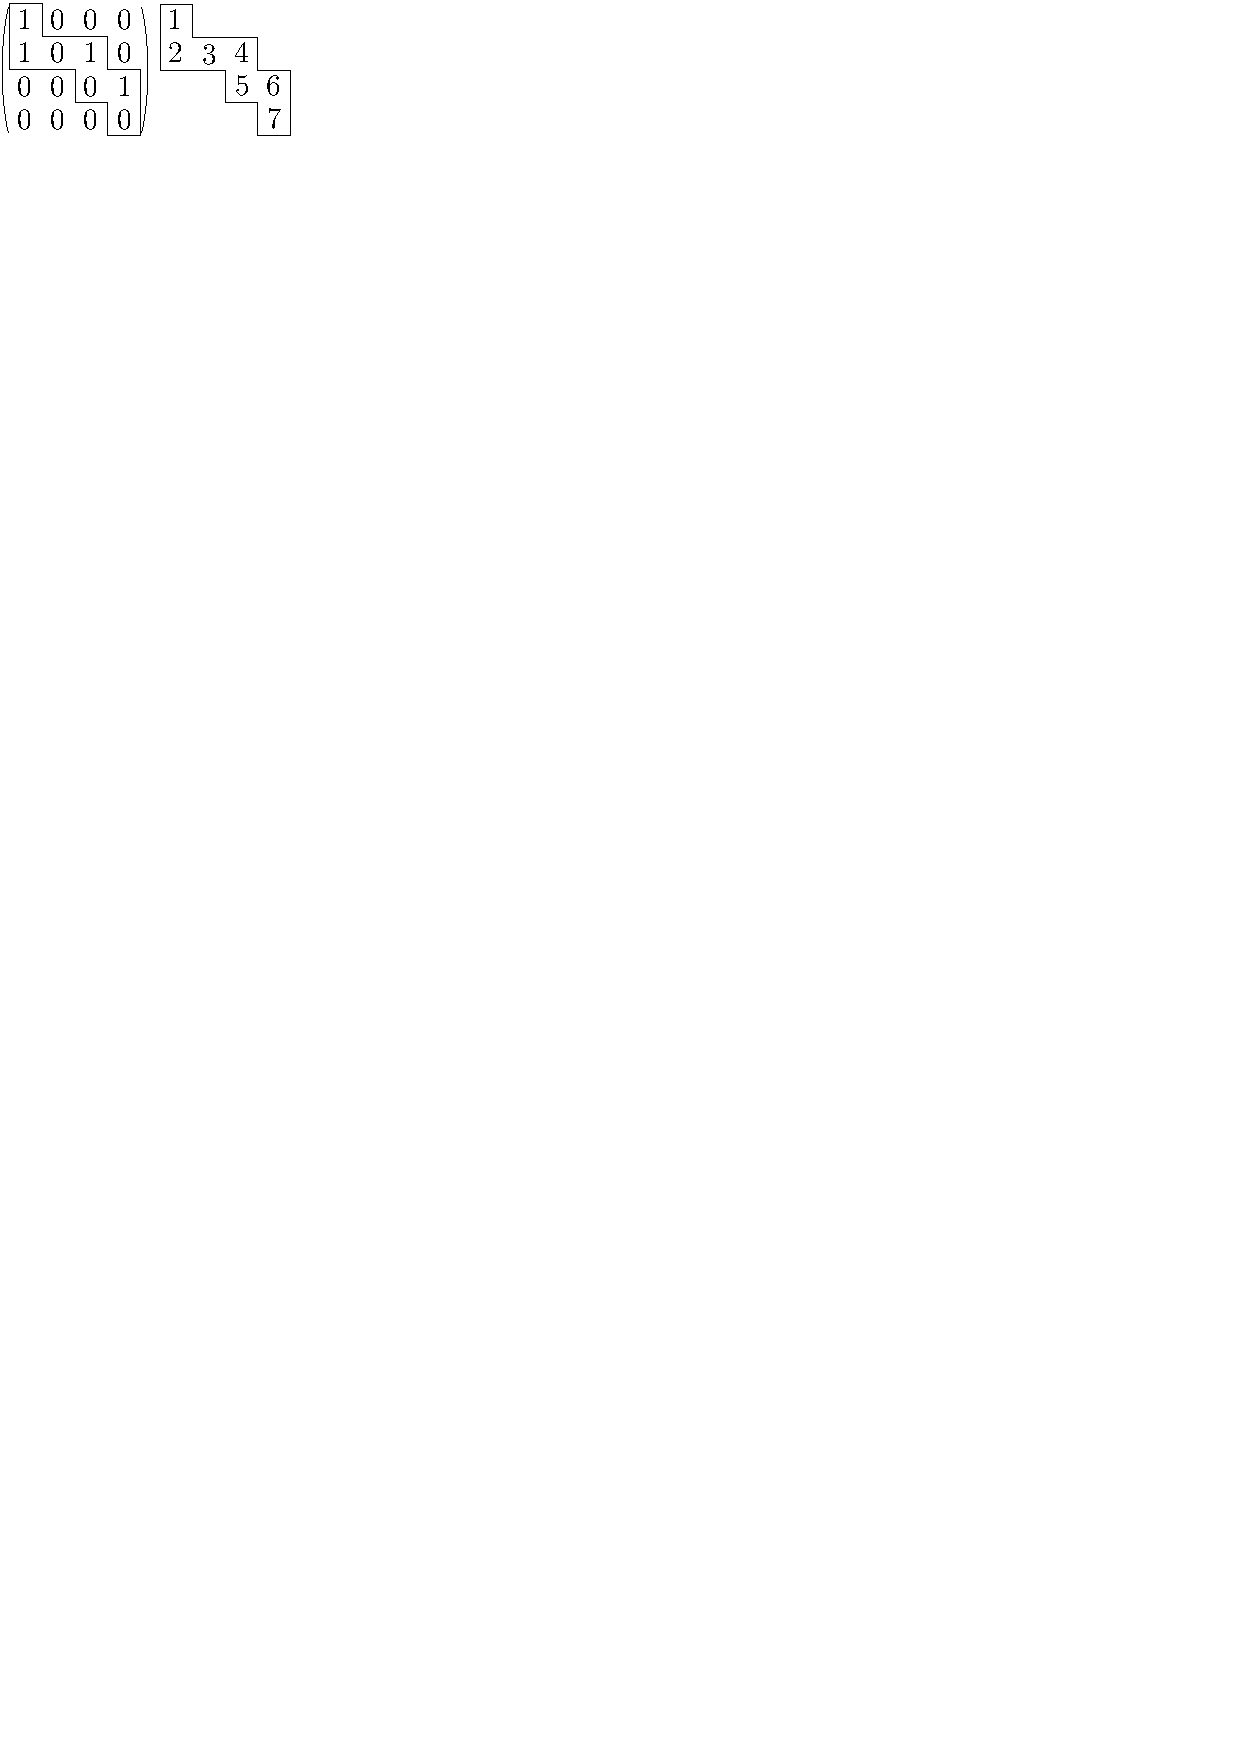
\includegraphics[width=75mm]{../img/walk.pdf}}}

In Figure \ref{walk} you can see a matrix that is a walking pattern as all the one-entries are included in a walk. Not all entries of a walk need to be one-entries though.

It can be shown a walking pattern with a walk is exactly a matrix avoiding a forbidden pattern
$$\left(\begin{array}{cc}
0 & 1 \\
1 & 0
\end{array}\right)$$

\section{Dynamic program}
Now that we know what walking pattern is, we show an algorithm deciding whether such a pattern $P$ is contained in a big matrix $M$ or not.

The pattern $P$ is a walking pattern so there is a walk containing all the one-entries of the pattern. We choose one such walk arbitrarily and index its entries $e_1,e_2,\dots,e_{h+w-1}$ starting from the beginning of the walk. For each entry of the walk we remember whether its value is one or zero and whether the walk continues from the entry vertically, in which case we call it a \textbf{vertical entry} or horizontally, calling it a \textbf{horizontal entry}.

For an element $e$ of $M$ at the position $[i,j]$, the matrix $M_{\leq e}$ is a $(i+1)\times(j+1)$ submatrix of $M$ consisting of rows with the index smaller than or equal to $i$ and columns with the index smaller than or equal to $j$. The element $e$ then lies in the bottom right corner. Similarly, $M_{\geq e}$ is a $(n-i)\times(n-j)$ submatrix of $M$ consisting of rows with the index greater than or equal to $i$ and columns with index greater then or equal to $j$. The element $e$ is its first element.

To determine whether $P$ is contained in $M$ we find out for each element $e$ of $M$ what is the longest part of the pattern that can be found in $M_{\leq e}$. If there is an element for which we manage to find the last entry of the pattern, the pattern is contained in the matrix; otherwise, it is avoided.

For each element $e$ of $M$ at the position $[i,j]$ we remember two numbers. The number $c_v(e)$ says what is the longest part of the walk in $M_{\leq e}$ with the last entry in $j$-th column and being a vertical entry. The number $c_h(e)$, symmetrically, says what is the longest part of the walk in $M_{\leq e}$ with the last entry in $i$-th row and and being a horizontal entry.

An observation we make is that if we have a fixed element $e$ of $M$ and any other element $e'$ above $e$ in the same column then $c_v(e')$ is less than or equal to $c_v(e)$. This means that for $e$ we can find the maximum part of the pattern ending in the column of $e$ and continuing vertically by looking only to elements in that column above $e$ and since this is true for all of them, it is sufficient to only check the value of the element right above $e$ (at the position $[i-1,j]$). Similarly the argument goes for the value of $c_h$ in horizontal way.

The algorithm iterates through diagonals. A diagonal in this matter of speaking is a subset of elements of $M$, such that all elements have the same sum of their coordinates. For example, zero diagonal only consists of an element $[0,0]$, the first diagonal contains elements $[0,1]$ and $[1,0]$, and so on.

For simplicity, in the pseudo-code below we do not deal with elements outside $M$ (like $-1,0$) explicitly. Instead for those elements we just assume the values of $c_v$ and $c_h$ are always equal to zero.

\subsection{The algorithm}
\begin{enumerate}
\item For $d=0,\cdots,w+h-1$
\item \hspace{5mm} For $e$ element of $d$-th diagonal at the position $[i,j]$
\item \hspace{1cm} $e_v:=[i-1,j]$
\item \hspace{1cm} $e_h:=[i,j-1]$
\item \hspace{1cm} $c_v(e):=c_v(e_v)$
\item \hspace{1cm} $c_h(e):=c_h(e_h)$
\item \hspace{1cm} If $w_{c_v(e)+1}$ can be mapped to $e$
\item \hspace{15mm} If $c_v(e)+1=w+h+1$
\item \hspace{2cm} Terminate - $M$ contains $P$ as a submatrix
\item \hspace{15mm} If $w_{c_v(e)+1}$ is a vertical entry
\item \hspace{2cm} $c_v(e):=c_v(e)+1$
\item \hspace{15mm} Else
\item \hspace{2cm} $c_h(e):=max\{c_h(e),c_v(e)+1\}$
\item \hspace{1cm} If $w_{c_h(e)+1}$ can be mapped to $e$
\item \hspace{15mm} If $c_h(e)+1=w+h+1$
\item \hspace{2cm} Terminate - $M$ contains $P$ as a submatrix
\item \hspace{15mm} If $w_{c_h(e)+1}$ is a vertical entry
\item \hspace{2cm} $c_v(e):=max\{c_v(e),c_h(e)+1\}$
\item \hspace{15mm} Else
\item \hspace{2cm} $c_h(e):=max\{c_h(e),c_h(e)+1\}$
\end{enumerate}

\centerline{\mbox{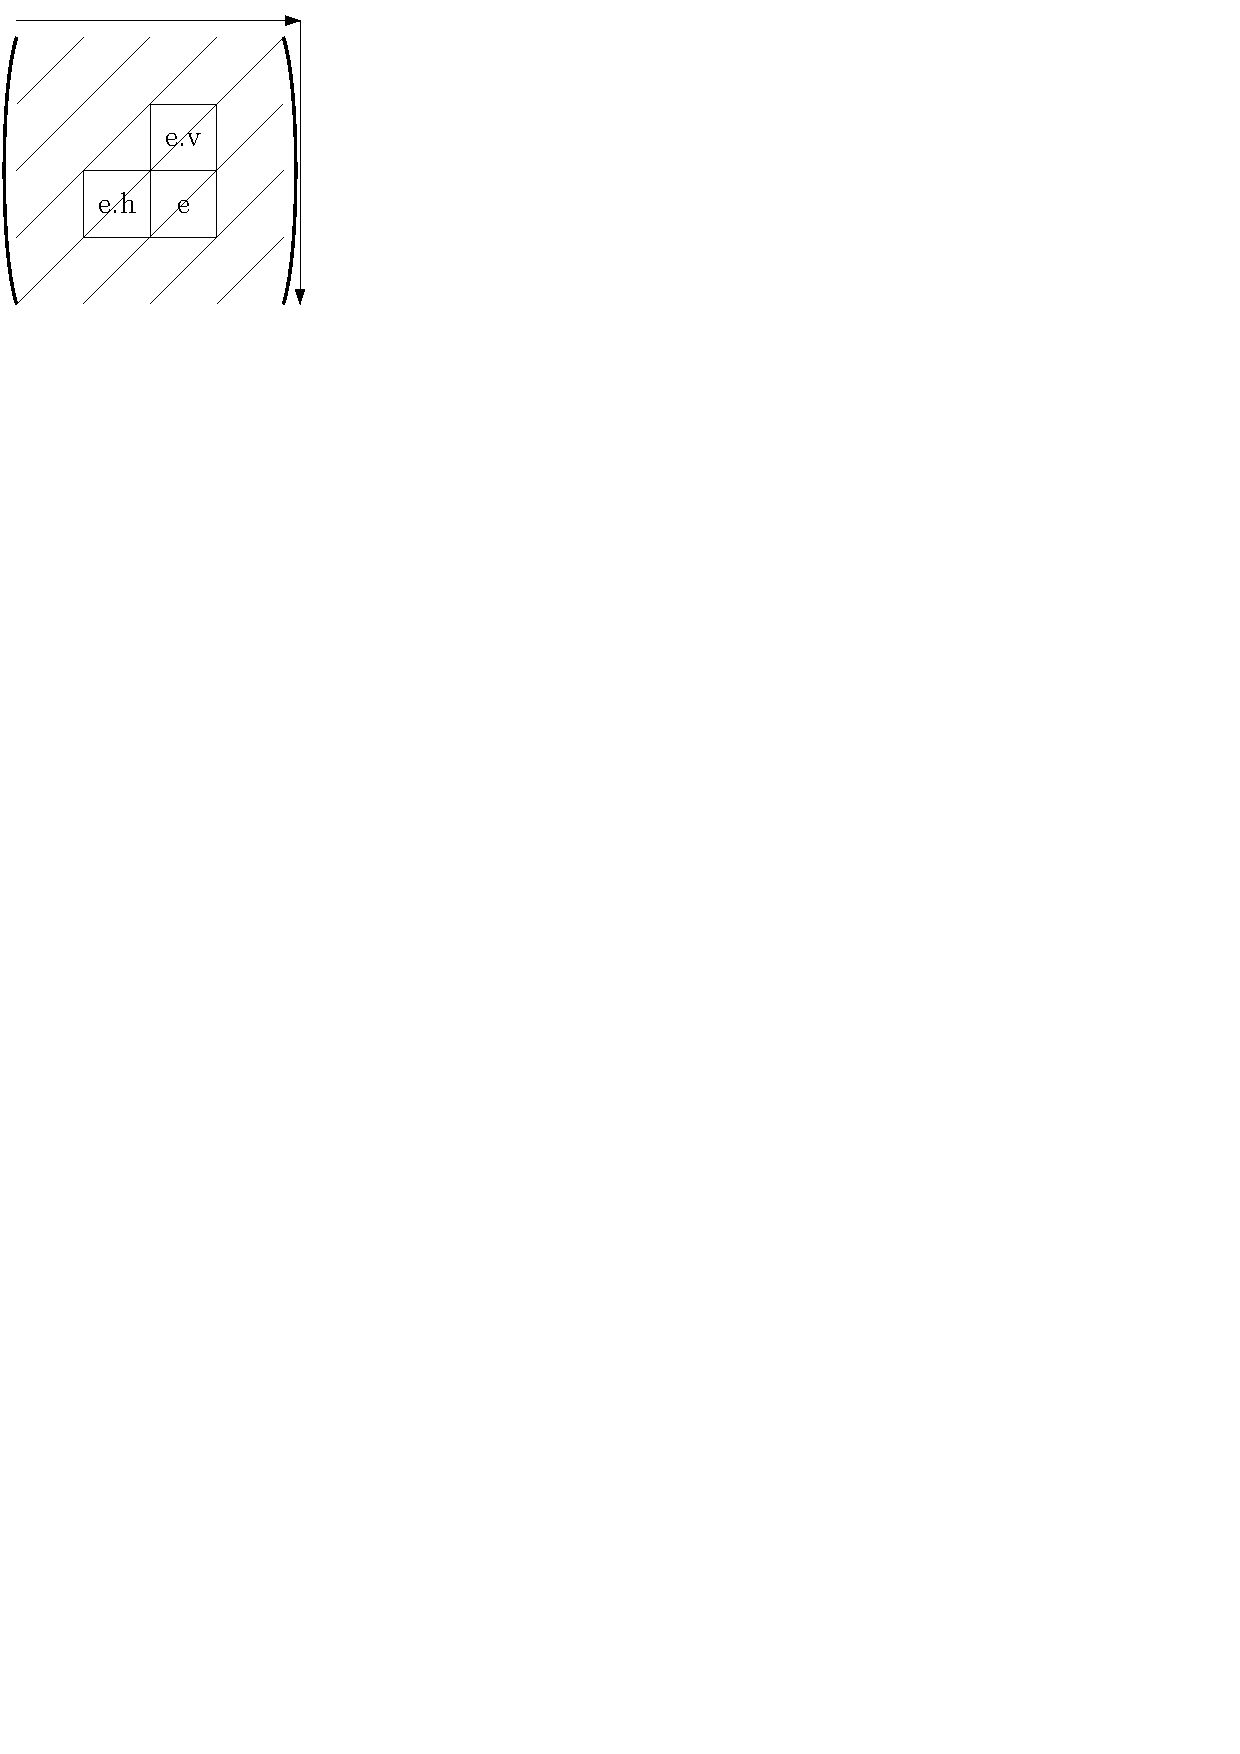
\includegraphics[width=60mm]{../img/walking_alg.pdf}}}

\subsection{Inner structure}
To run properly the algorithm needs two structures. The first one is a description of the walk, which is just an array of the values of its entries as well as the information whether the entry is vertical or horizontal. The second structure is a matrix of the values $c_v$ and $c_h$ as described above.

\subsection{Correctness}
We need to show that the values of $c_v$ and $c_h$ are always correct for the recomputed elements after at the end of the function. We proceed by induction.

For the first element it is definitely true since there can be only the first entry of the pattern mapped and we check just that.

When we compute an element $e$ of a computed diagonal $d$, by induction assumption all the diagonals $d'<d$ are correctly computed. In particular, the values are correct in the diagonal $d-1$. To compute the correct values of $e$, we use the values of two element on the diagonal $d-1$: $e_v$, which is right above $e$ and $e_h$, which is the first element to the left of $e$. If $e_v$ or $e_h$ are outside the matrix then from that direction we cannot expect to find anything more than just the first entry of the pattern and that is what we check for.

Let $v$ be the true length of the longest part of $P$ in $M_{\leq e}$ continuing vertically in the same column as $e$. Now if $e$ itself is not an entry of that part of the pattern, it is a different element $e'$ in the same column. But then the value of $c_v(e')$ is correctly computed by the inductive hypothesis and it is copied to all element underneath. Especially $e_v$ gets the value and the algorithm copies the value from it to $e$. On the other hand if $e$ is an entry of the part of the pattern we work with, it is the last entry. The entry right before the last one needs to be mapped to the same row or column; therefore, either $e_v$ or $e_h$ contain the part of the pattern shorter by one and the algorithm extends it to a correct value.

\subsection{Generalization}
The same algorithm, just rotated by 90 degrees, can be also used for a pattern where all one-entries are contained on a walk from top right corner to the bottom left one. Indeed the program uses it and if given a walking pattern it determines by itself which walk it is.

On the other hand a direct generalization for a general pattern does not work. While we can index all entries of the pattern, when trying to map a certain $w_k$ to an element it is not sufficient to just check whether $w_l$ is above and $w_l'$ to the left from the element.

\centerline{\mbox{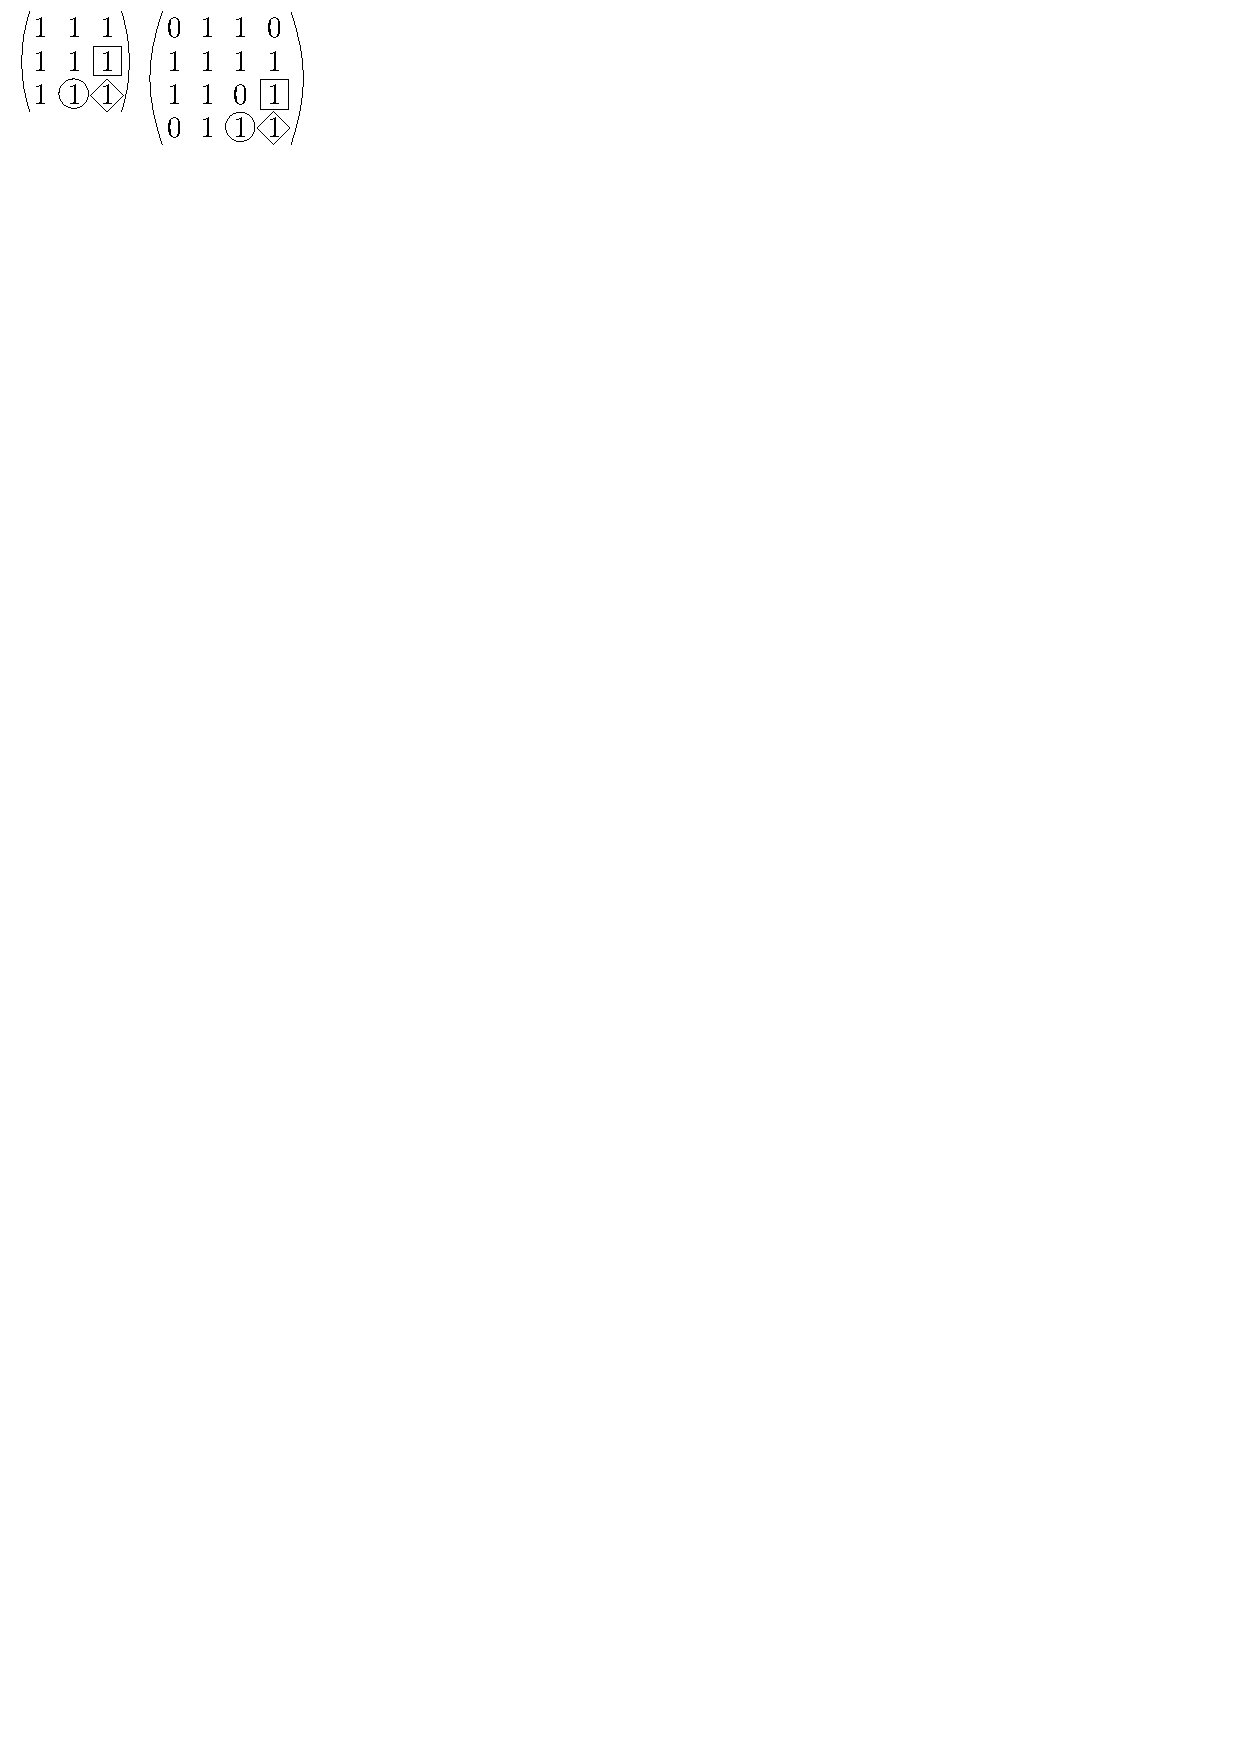
\includegraphics[width=75mm]{../img/nogeneral.pdf}}}

In the picture, let the matrix on the left side be the pattern $P$ and let $M$ be the other matrix. The entry in the square can be mapped to the element in the square and the same holds for entries in the circle but it is not a sufficient condition for the entry in the triangle to be mapped to the element in the triangle.